\documentclass[10pt,twocolumn]{article}
\usepackage[a4paper,margin=1.8cm,columnsep=0.6cm]{geometry}
\usepackage[T1]{fontenc}
\usepackage{lmodern,microtype}
\usepackage{amsmath,amssymb,bm}
\usepackage{graphicx,booktabs,array,xcolor,colortbl,tabularx}
\usepackage[numbers,sort&compress]{natbib}
\usepackage[hidelinks]{hyperref}
\usepackage{tikz}
\usetikzlibrary{arrows.meta,positioning,fit,calc}
\usepackage{caption}
\captionsetup{font=small,labelfont=bf}
\usepackage{enumitem}
\setlist{nosep,leftmargin=*}
\definecolor{keybg}{RGB}{238,244,250}
\newcommand{\R}{\mathcal{R}}

\title{\vspace{-1.2em}\textbf{Cross-Examined Fusion: Earning Trust by Corroboration in Multimodal Uncertainty}\\[2pt]
\large Final Year Project, Part II --- Research Proposal}
\author{\small Builds on Part I (\emph{Does the Uncertainty Notice?}). Code: \url{https://github.com/fasihh/bigthing} (\texttt{JF/})}
\date{\small November 2026}

\begin{document}
\maketitle

\begin{abstract}
Part~I found that a product of probabilistic experts handles a \emph{declared} missing modality well, but is blind to a
\emph{silently} broken one. Each expert's uncertainty is computed from its own input, so an expert fed pure noise or
another clip's data stays confident (sensor-swap detection AUROC 0.50, text share of the fusion 0.89 under pure noise,
90\% coverage falling to 0.75--0.80). We propose \textbf{Cross-Examined Fusion (CXF)}: a modality's weight should be
\emph{earned by being corroborated by the other senses, not self-reported}. CXF fits a joint density of frozen,
label-free JEPA beliefs on clean data only. At test time it computes an exact posterior over which senses are lying
($2^M$ hypotheses) and fuses by Bayesian model averaging over the trusted subsets. A corrupted sense is then treated
as \emph{inferred missing}, so the missing-modality machinery that already works, including per-subset conformal
calibration, applies to corruption without ever seeing corrupted data. A secondary contribution,
\textbf{Persistence Targets}, addresses the one failure CXF cannot see: a nuisance shared by every sense, which
hijacks self-predictive objectives. We evaluate on CMU-MOSEI and, as a second and very different benchmark, on
MS-COCO (an image plus two independent captions), against classical fault-detection, deep reliability and conformal
baselines. A one-week go/no-go pilot on existing checkpoints decides the scope before any new training.
\end{abstract}

\section{Motivation: what Part I established}
\begin{table}[h]
\centering\small
\colorbox{keybg}{\parbox{0.96\columnwidth}{\centering
\textbf{Part I numbers this proposal attacks} (CMU-MOSEI, 3 seeds)\\[2pt]
\resizebox{0.94\columnwidth}{!}{\begin{tabular}{@{}l r@{}}
Tracking ratio, text \emph{declared} missing (PoE) & 1.007 \;(ideal 1)\\
Tracking ratio, text \emph{silently} pure noise & 0.63--0.86\\
Text expert $\sigma$ as its input becomes noise & 0.068 $\to$ 0.061 (falls)\\
Text share of fused precision under pure noise & 0.89\\
Cov90, text pure noise (fine-tuned, rescaled) & 0.746 \;(target 0.90)\\
Swap detection AUROC by $\sigma$ & 0.49--0.55\\
Swap detection by disagreement, frozen / fine-tuned & up to 0.87 / 0.50\\
Precision given to a pure-noise modality & 13--38\%\\
Signal $R^2$ under a shared sticky distractor & 0.33 $\to$ 0.07
\end{tabular}}}}
\end{table}
Part~I compared four pretraining objectives, three regimes and four fusion rules over 46 test conditions. Two
mechanisms explain its failures. (i)~\emph{Self-reported trust}: in a PoE an expert's weight is its own precision,
which it computes from its own (possibly broken) input. A Gaussian head trained on clean data maps unfamiliar
input to a familiar, confident belief~\cite{kendall2017uncertainties}. (ii)~\emph{What is corroborated is not always
content}: a self-predictive target keeps whatever is predictable, including a nuisance shared by all modalities.
The information needed to notice a broken sense exists: frozen experts' disagreement detects swaps with AUROC up
to 0.87. But PoE does not use it, and fine-tuning erases it.

\section{Related work and novelty}
\paragraph{The principle is classical.} Detecting and isolating a faulty sensor from cross-sensor consistency is
\emph{analytical redundancy}: parity relations and generalized voting~\cite{chow1980failure}, banks of fault hypotheses
with posterior probabilities (multiple-model adaptive estimation)~\cite{roumeliotis1998fault}, and per-sensor outlier
indicators in robust fusion~\cite{wang2022outlier}. CXF is \emph{this idea rebuilt inside a learned latent world
model}; we do not claim a new principle.
\paragraph{Deep reliability-aware fusion.} An odd-one-out network weights leave-one-out fusions by the probability
that each modality is perturbed~\cite{yang2021defending}, and quality heads are regressed to injected corruption
severity~\cite{kumar2026prime,wu2026electronics}: all are \emph{trained on corruptions}. Reliability-weighted PoE learns
a sigmoid weight from task labels alone; its authors note that learning dependable quality signals remains an open
challenge~\cite{palo2026reliability}. Conflict discounting~\cite{bezirganyan2025discounted}, generalized
PoE~\cite{cao2014gpoe} and circuit-based credibility~\cite{tenali2026c2mf} re-weight beliefs by fixed or supervised rules.
\paragraph{Corruption-free detection.} Several methods need no corrupted training data. A PoE trained with modality
dropout can drop an expert flagged by its own reconstruction error~\cite{lee2020detect}; clean-only per-stream detectors
can swap flagged streams for the missing-modality token~\cite{mohapatra2026carat}; world-model surprise can select a
trusted sensor subset~\cite{zollicoffer2025wiser}; cross-modal reconstruction can flag faults~\cite{jensen2026fault}; and
clean-only multi-view densities can flag inconsistent views~\cite{wang2020hbmvad}. These detectors are either unimodal
(so they cannot see a realistic but mismatched sense) or unlocalised, and all make hard decisions without calibrated
predictive uncertainty.
\paragraph{Conformal.} Per-missingness-pattern (Mondrian) conformal calibration exists for multimodal
regression~\cite{azizi2026conformal,mccf2026}, but it assumes the pattern is known.

\paragraph{What is new in CXF.}
\begin{enumerate}
\item An \emph{exact} posterior over all $2^M$ corruption configurations from a \emph{cross-modal conditional} density
  of frozen JEPA beliefs fitted on clean, unlabelled data. Because the evidence is conditional, it can catch swapped or
  mismatched senses that unimodal clean-only detectors miss by construction.
\item \emph{Soft} corruption-as-missingness: Bayesian model averaging of the predictive densities of all trusted
  subsets, rather than a hard reject~\cite{lee2020detect,mohapatra2026carat}.
\item Per-pattern conformal intervals mixed by the posterior, so intervals calibrated only on declared missingness are
  reused under inferred corruption; coverage under corruption is measured empirically.
\item The empirical finding that fine-tuning erases cross-modal agreement, and an auditor/worker split that keeps it.
\item The first evaluation of multimodal \emph{regression} under silent corruption, including swaps, by coverage, CRPS
  and tracking ratio, on MOSEI and an image-plus-two-captions COCO benchmark (prior MOSEI reliability work reports
  classification calibration under injected corruption~\cite{wu2026electronics}).
\end{enumerate}
We do not claim the principle (analytical redundancy), clean-data-only fitting, hard corruption-to-missing conversion,
or latent world-model surprise as new.

\section{Method: Cross-Examined Fusion}
\begin{figure}[t]
\centering
\resizebox{\columnwidth}{!}{%
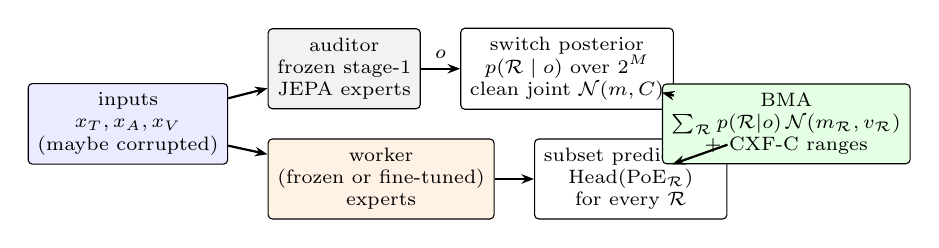
\begin{tikzpicture}[font=\scriptsize, node distance=3mm,
  box/.style={draw, rounded corners=1.5pt, minimum height=5mm, align=center, fill=white},
  arr/.style={-{Stealth[length=1.6mm]}, thick}]
\node[box, fill=blue!8] (x) {inputs\\$x_T,x_A,x_V$\\(maybe corrupted)};
\node[box, right=5mm of x, yshift=7mm, fill=gray!10] (aud) {auditor\\frozen stage-1\\JEPA experts};
\node[box, right=5mm of x, yshift=-7mm, fill=orange!10] (wrk) {worker\\(frozen or fine-tuned)\\experts};
\node[box, right=5mm of aud] (post) {switch posterior\\$p(\R\mid o)$ over $2^M$\\clean joint $\mathcal N(m,C)$};
\node[box, right=5mm of wrk] (sub) {subset predictions\\$\mathrm{Head}(\mathrm{PoE}_\R)$\\for every $\R$};
\node[box, right=8mm of $(post)!0.5!(sub)$, fill=green!10] (bma) {BMA\\$\sum_\R p(\R|o)\,\mathcal N(m_\R,v_\R)$\\+ CXF-C ranges};
\draw[arr] (x) -- (aud); \draw[arr] (x) -- (wrk);
\draw[arr] (aud) -- node[above]{$o$} (post); \draw[arr] (wrk) -- (sub);
\draw[arr] (post) -- (bma); \draw[arr] (sub) -- (bma);
\end{tikzpicture}}
\caption{Cross-Examined Fusion. The auditor never sees labels or corruptions; the worker is any Part~I PoE model.}
\label{fig:cxf}
\end{figure}

\paragraph{Evidence.} For clip $x$ and modality $m$, the frozen auditor gives a belief mean $\bm\mu^{A}_m(x)$.
Optionally it also gives the modality's own target latent $\bm e_m(x)$. A PCA fitted on clean training latents
summarises them in $k=8$ dimensions: $o_m=P_m\bm\mu^A_m$ (plus $Q_m\bm e_m$), and $o=[o_1,\dots,o_M]$.

\paragraph{Clean joint density.} Fit $o\sim\mathcal N(m,C)$, with shrinkage, on half of the \emph{clean, unlabelled}
validation set.

\paragraph{Switch posterior.} Each modality has a switch $c_m\in\{0,1\}$, where 1 means ``lying'', with prior
$\pi=0.05$. With reliable set $\R=\{m:c_m=0\}$,
\begin{equation}
p(o\mid c)=\mathcal N(o_\R;m_\R,C_{\R\R})\prod_{m\notin\R}\mathcal N(o_m;m_m,\kappa C_{mm}),
\end{equation}
so a lying block is decoupled from the others and broadened ($\kappa=10$). The posterior over all $2^M$ configurations
is exact:
$\log p(c\mid o)=\tfrac1T\log p(o\mid c)+\sum_m\log\pi^{c_m}(1-\pi)^{1-c_m}+\text{const}$. The temperature $T$ is set on the
other clean validation half so that the clean false-alarm rate is 1\%. Holding the other switches at ``reliable'', the
log Bayes factor for ``$m$ is lying'' is $\tfrac1{2T}[d^2_{\text{cond}}(m)-d^2_{\text{marg}}(m)/\kappa]+\text{const}$.
Here $d^2_{\text{cond}}$ is the distance of block $m$ from its \emph{linear prediction by the other senses}: a learned,
calibrated version of a parity relation~\cite{chow1980failure}. A swapped sense looks normal on its own but not
conditionally. A pure-noise sense is surprising both ways.

\paragraph{Prediction by model averaging.} The Part~I worker was trained on random modality subsets, so the
prediction from every subset, $(m_\R,v_\R)=\mathrm{Head}(\mathrm{PoE}_\R)$, is in-distribution. CXF reports
\begin{equation}
p(y\mid x)=\sum_\R p(\R\mid o)\,\mathcal N(y;m_\R,v_\R).
\end{equation}
Its variance includes the spread between subsets, and $r_m=P(c_m=1\mid o)$ is a label-free corruption probability.
\textbf{CXF-C} mixes per-subset conformal intervals, calibrated on clean data with \emph{declared} missing subsets, by
$p(\R\mid o)$. If the posterior is right, a corrupted clip is calibrated as if the sense were missing.

\paragraph{Why exact inference, not a learned weight or a hard reject.} A learned residual-to-weight map needs labels or injected
corruptions, which puts it in the crowded corruption-supervised family. The exact posterior needs only clean data,
gives testable probabilities, and yields subset-level mixing, hence CXF-C. The learned map is kept as an ablation
and a baseline.

\paragraph{Phase B: trained witnesses.} If the pilot shows that the audio--video relations are too weak, train
per-modality EMA targets and $M\times M$ cross-modal predictor heads, so that every pair of senses has a learned
relation. The fusion space and the workers are unchanged.

\begin{table*}[!t]
\centering\small
\caption{Hypotheses with measurable success criteria. ``Part I'' values are from the 3-seed MOSEI run; targets are 5-seed means
whose 95\% bootstrap interval excludes the Part~I value. FR = frozen V-JEPA PoE worker; FT = fine-tuned worker with a frozen auditor.}
\label{tab:hyp}
\setlength{\tabcolsep}{4pt}
\footnotesize\begin{tabularx}{\textwidth}{@{}l >{\raggedright}X >{\raggedright}p{3.6cm} >{\raggedright}p{3.3cm} >{\raggedright\arraybackslash}p{3.0cm}@{}}
\toprule
\# & Hypothesis & Metric & Part I & Target\\
\midrule
H1 & CXF detects alien input that $\sigma$ cannot see & AUROC of $r_T$, text pure noise & $\sigma$: $\approx$0.50 & $\geq$0.90\\
H2 & CXF localises swaps \emph{better than raw disagreement} (the real test) & AUROC of $r_A$, $r_V$; localisation & disagreement 0.56 (V-JEPA) / 0.84 (align) & $\geq$0.70 / $\geq$0.85 and $\geq$+0.03\\
H3 & Repairs accuracy under corruption & MAE, text pure noise & FR 0.848, FT 0.870 & FR $\leq$0.83, FT $\leq$0.84\\
H4 & Repairs coverage without corrupted calibration data & Cov90, text pure noise & FR 0.799, FT 0.746 & $\geq$0.86 raw, $\geq$0.88 CXF-C\\
H5 & Fusion weight and $\sigma$ follow corruption & text share; tracking ratio & 0.89; 0.86 / 0.63 & $\leq$0.25; 0.95--1.10\\
H6 & A pure-noise sense gets no weight, without labels & precision share of the noise sense & 0.13--0.38 & $\leq$0.05\\
H7 & No harm on clean data & MAE / NLL / Cov90; false-alarm rate & FT 0.563 / 1.261 / 0.883 & $\leq$+0.005 / +0.01 / $\pm$0.01; FAR $\leq$2\%\\
H8 & Persistence Targets resist the shared distractor & signal / distractor $R^2$, $\sigma=8$ & 0.068 / 0.517 & $\geq$0.20 / $\leq$0.15\\
H9 & Persistence transfers to Huang's toy & distractor $R^2$ vs VJEPA, 15 seeds & --- & better in $\geq$12/15 seeds\\
H10 & The findings replicate on MS-COCO & H1, H2, H4, H7 metrics & --- & same direction; H1 $\geq$0.85\\
\bottomrule
\end{tabularx}
\end{table*}

\subsection{Secondary contribution: Persistence Targets}
CXF trusts what the senses agree on. A distractor shared by all senses makes them agree on the nuisance. In Part~I
this hijacked every self-supervised objective (signal $R^2$ 0.33$\to$0.07, distractor $R^2$ 0.52). The \emph{target}
must change. A Persistence Target is something that a \emph{different modality} can predict from a
\emph{distant time window} of the clip. A sticky but short-lived nuisance cannot cross the time gap; a lasting nuisance
confined to one sense cannot cross the modality gap. This follows within-clip persistence ideas in video
self-supervision~\cite{feichtenhofer2021largescale} and the slow-noise analysis of~\cite{gulati2026contrast}. The
auditor trained this way becomes the ``persistence witness'' for CXF. \emph{Stated limit:} a nuisance that is lasting,
shared and predictable cannot be separated from content without labels.

\subsection{Stretch: Time Auditor}
With $M=3$, CXF cannot distinguish ``two senses lie'' from ``the third lies''. A within-modality block, the surprise of
masked-frame prediction inside the clip, breaks the tie, because it does not depend on the other senses.

\section{Experimental plan}
\paragraph{Datasets.}
\textbf{CMU-MOSEI}~\cite{zadeh2018mosei}, as in Part~I.
\textbf{MS-COCO 2017}~\cite{lin2014coco}, a second and very different benchmark: three ``sensors'' per scene, namely the
image (DINOv2-small patch tokens~\cite{oquab2023dinov2}) and two captions from different annotators (MiniLM token
states~\cite{reimers2019sbert}). The task is regressing the number of annotated objects (log scale). Image and text
encoders are separately trained, so the senses are not pre-aligned. A mismatched caption is a natural, realistic
corruption. We use 20k training and 2.5k validation images from train2017, and the 5k val2017 images as test.
\textbf{CMU-MOSI}~\cite{zadeh2016mosi} (same features as MOSEI) is a third check, if time permits.

\paragraph{Corruptions.} The Part~I suite: missing subsets; test-time noise $\lambda\in\{0.5,1\}$ on each sense; swapped
sense; an extra pure-noise sense; a shared or independent sticky distractor. None of these is used to fit CXF.

\paragraph{Baselines.}
(1)~Part~I fusions: PoE, prior-corrected PoE, MoE, attention, concatenation, late averaging, MoNIG~\cite{ma2021monig},
robust and disagreement-aware PoE.
(2)~Classical fault detection: a $\chi^2$ innovation gate; variational Bernoulli outlier indicators~\cite{wang2022outlier};
a hypothesis bank with identity covariance (CXF without learned relations).
(3)~Deep reliability: gPoE~\cite{cao2014gpoe}, conflict discounting~\cite{bezirganyan2025discounted}, reliability-weighted
PoE~\cite{palo2026reliability}, and odd-one-out fusion~\cite{yang2021defending} trained on some corruption families and
tested on others (reported separately as corruption-supervised).
(4)~Conformal: split, per-mask (Mondrian)~\cite{azizi2026conformal}, disagreement-scaled.
(5)~\textbf{Corruption-free detectors (the decisive comparison):} a Lee/CARAT-style hard drop (clean-only per-modality
Mahalanobis detector, flagged modality set to missing, its per-mask interval)~\cite{lee2020detect,mohapatra2026carat};
CXF with a hard most-likely subset instead of averaging; WISER-style lowest-surprise subset
selection~\cite{zollicoffer2025wiser}; and a reconstruction-evidence variant of CXF, to test whether JEPA beliefs
matter~\cite{jensen2026fault}. CXF must beat the hard drop on swaps (H2) and on coverage (H4).



\paragraph{Ablations.} Evidence blocks (beliefs only; own target; both; time block). Covariance (learned vs identity
vs diagonal). Inference (exact model averaging vs soft precision scaling vs MAP subset vs learned map). Likelihood
(Gaussian vs Student-$t$). Hyperparameters ($\pi$, $\kappa$, $k$, false-alarm target), reported as a sensitivity grid,
not tuned. Auditor (frozen V-JEPA vs alignment vs no split).

\paragraph{Week-1 go/no-go pilot (no training).} The code is ready (notebook 09). It uses frozen Part~I experts and
stage-2 models, fits on clean validation halves, and scores on test.
\textbf{G1}: AUROC$(r_T)\geq0.90$ under text noise with clean false-alarm rate $\leq2\%$.
\textbf{G2}: swap AUROC $\geq0.70$ \emph{and} at least 0.03 above that auditor's raw disagreement.
\textbf{G3}: on the fine-tuned worker under text noise, Cov90 $\geq0.83$ (from 0.746) and MAE $\leq0.85$ (from 0.870),
with clean MAE worse by at most 0.005.
All three pass: GO. G2 fails: GO-narrow, Phase B becomes mandatory. G1 fails: NO-GO, switch to the fallback.
G1 alone could be met by any single-modality OOD score, so the scientific claim rests on G2 and H4. A
``marginal-only'' ablation is reported next to CXF everywhere.

\paragraph{Compute.} Free Kaggle T4 GPUs (about 30 GPU-h per week). CXF itself is inference-only: $2^M=8$ small
Gaussian evaluations and 8 cheap subset predictions per batch. The estimated total for the plan, including a $2\times$
margin for re-runs, is about 220 GPU-h over 26 weeks, against about 780 available. Week~1 replaces the estimates with
measured times.

\begin{table}[t]
\centering\small
\caption{Timeline (26 weeks).}
\resizebox{\columnwidth}{!}{%
\begin{tabular}{@{}ll@{}}
\toprule
Weeks & Work and decision\\
\midrule
1 & Go/no-go pilot on Part~I checkpoints; measure run times\\
2--4 & CXF and all baselines; MOSEI, 3 seeds; first H1--H7 numbers\\
5--6 & CXF-C conformal; ablations; seeds 3--4 \;\textbf{(mid-term table)}\\
7--8 & MS-COCO replication (H10); corruption-supervised baselines\\
9--12 & Phase B trained witnesses (if GO-narrow, earlier)\\
13--17 & Persistence Targets: MOSEI distractor grid, Huang toy (H8--H9)\\
18--20 & Stretch: Time Auditor, or CMU-MOSI\\
21--22 & Freeze; final 5-seed tables; failure analysis\\
23--26 & Writing, figures, viva; 2-week buffer\\
\bottomrule
\end{tabular}}
\end{table}

\section{Risks and fallback}
\begin{itemize}
\item \textbf{Weak cross-modal information} (MOSEI audio and video are weak, AV-only MAE 0.81): swaps may stay
  undetectable with the V-JEPA auditor. Mitigations: test the alignment auditor (disagreement AUROC 0.84 in Part~I),
  Phase B, and MS-COCO, where two captions describe the same scene.
\item \textbf{Attractor effect}: a corrupted input may map onto the clean manifold in latent space. Mitigations: the
  own-target block, the time block, or fallback F1.
\item \textbf{Misspecified Gaussian}: the temperature is set by the clean false-alarm rate; a Student-$t$ ablation is
  included.
\item \textbf{Two-of-three ambiguity} is certain in principle, and is reported as an identifiability limit.
\item \textbf{``This is just fault detection'' or ``just Lee et al./CARAT with a soft posterior''}: we cite them up
  front, claim only the deltas in Section~2, and include the identity-covariance hypothesis bank and the hard-drop
  baselines. The decisive evidence is swaps: unimodal clean-only detectors cannot detect them by construction.
\end{itemize}
\textbf{Fallbacks.} F1: keep the inference engine, use input-level evidence (Time Auditor). F2: promote Persistence
Targets to the headline, with CXF as a quantified negative result. F3: a minimum viable contribution, the first
coverage/CRPS/tracking benchmark of more than 15 reliability-fusion methods under corruption on MOSEI and COCO.

\section{Expected outcome}
A fusion rule whose trust in each sense comes from the other senses, so that a silently broken input is treated like
a missing one. Its measurable promise: detection AUROC from 0.5 to above 0.9, coverage under corruption from
0.75 to above 0.86, and no cost on clean data, all without corrupted training data. It is evaluated on two very
different multimodal benchmarks, against classical and deep baselines.

{\small
\bibliographystyle{unsrtnat}
\bibliography{refs}
}
\end{document}
